\documentclass[11pt,a4paper]{article}
\usepackage[utf8]{inputenc}
\usepackage[T1]{fontenc}
\usepackage[main=french,provide=*]{babel}
\usepackage[margin=2.3cm]{geometry}
\usepackage{graphicx}
\usepackage{amsmath,amssymb}
\usepackage{booktabs}
\usepackage{caption}
\usepackage{float}
\usepackage{enumitem}
\usepackage{natbib}
\usepackage[hidelinks]{hyperref}
\usepackage{titlesec}
\usepackage{fancyhdr}
\usepackage[protrusion=true,expansion=false]{microtype}
\usepackage{xcolor}
\emergencystretch=1.5em

\definecolor{dauphblue}{RGB}{30,70,120}
\providecommand{\og}{\guillemotleft\,}
\providecommand{\fg}{\,\guillemotright}
\titleformat{\section}{\large\bfseries\color{dauphblue}}{\thesection}{0.6em}{}
\titleformat{\subsection}{\normalsize\bfseries\color{dauphblue}}{\thesubsection}{0.6em}{}
\titleformat{\subsubsection}{\small\bfseries}{\thesubsubsection}{0.6em}{}
\captionsetup{font=small,labelfont=bf}
\setlength{\parskip}{0.32em}
\setlength{\parindent}{0pt}

\pagestyle{fancy}\fancyhf{}
\rhead{\small Climat et Banque Centrale}
\lhead{\small Politique Monétaire, Université Paris-Dauphine}
\cfoot{\thepage}
\renewcommand{\headrulewidth}{0.3pt}

\begin{document}

%================ PAGE DE GARDE ================
\begin{titlepage}
\centering
\vspace*{1.4cm}
{\small\textsc{Université Paris-Dauphine, PSL}\par}
{\small\textsc{Master Ingénierie Économique \& Financière}\par}
{\small Cours : Politique Monétaire, Macroéconomie et Allocation d'Actifs (R.~Aumond, U.~Dubois)\par}
\vspace{2.0cm}
\rule{\linewidth}{0.4pt}\\[0.5cm]
{\LARGE\bfseries\color{dauphblue} Climat : la Banque Centrale\\[0.2cm] a-t-elle un rôle à jouer ?\par}
\vspace{0.5cm}
{\large Une analyse économétrique de la \emph{climateflation}\\
par SVAR, Local Projections et allocation d'actifs\par}
\rule{\linewidth}{0.4pt}\\[1.4cm]
{\large\itshape Soutenance du 13 juin}\par
\vspace{2.2cm}
\begin{minipage}{0.9\textwidth}\centering
\textbf{Groupe 4}\\[0.3cm]
Yves-Marie \textsc{Saliou} \quad\textperiodcentered\quad Milos \textsc{Gajic} \quad\textperiodcentered\quad Marc \textsc{Jehannin}
\end{minipage}
\vfill
{\small Données et codes Python reproductibles fournis en accompagnement.\par}
{\small \today\par}
\end{titlepage}

%================ RESUME ================
\section*{Résumé}
\small
Le changement climatique pose une question directe aux banques centrales, dont le mandat
premier est la stabilité des prix : les aléas climatiques sont-ils une source d'inflation,
et si oui, justifient-ils une réponse de politique monétaire ? Nous abordons cette
question, celle de la \emph{climateflation}, au moyen de six exercices économétriques
articulés, sur données mensuelles américaines couvrant 1987 à 2026. D'abord, un SVAR à
identification récursive montre qu'un choc de température (un mois plus chaud que la tendance)
a, historiquement et au niveau agrégé, un effet faible et plutôt désinflationniste à
court terme sur l'inflation (moins de 3\,\% de sa variance), et un effet quasi nul sur l'activité.
Mis en regard, le canal \emph{fossilflation} (le prix du pétrole) explique
environ treize fois plus de variance d'inflation que le canal climatique, ce qui quantifie
le diagnostic de \citet{schnabel2022}. Des Local Projections révèlent ensuite une
intensification : la réponse de l'inflation à moyen terme est devenue
significativement plus positive depuis 2007 (de $+1{,}0$ à $+1{,}4$ pp, $t$ jusqu'à $2{,}5$).
Cet effet est par ailleurs fortement asymétrique : les chocs chauds
deviennent inflationnistes à moyen terme tandis que les chocs froids restent désinflationnistes.
Du côté de l'allocation d'actifs, les obligations sont la classe la plus exposée
négativement, l'or servant de couverture ; neutraliser l'exposition climatique
coûte $13{,}6\,\%$ de ratio de Sharpe. Ces conclusions résistent enfin à des variations de
l'ordre de Cholesky, du nombre de retards et de la méthode de détrendage. Au total, la
banque centrale a bien un rôle, mais principalement \emph{prospectif} et de \emph{gestion
des risques} (supervision, stabilité financière, cadre de garanties) plutôt que comme cible
directe d'inflation.
\normalsize

\tableofcontents
\vspace{0.3cm}

%================ 1. INTRODUCTION ================
\section{Introduction et problématique}
En mars 2022, Isabel Schnabel (BCE) distingue trois canaux par lesquels le climat nourrit
l'inflation \citep{schnabel2022} : la \emph{climateflation}, où les aléas climatiques
perturbent l'offre (agriculture, énergie, logistique) ; la \emph{fossilflation}, soit le coût
d'une dépendance persistante aux énergies fossiles ; et la \emph{greenflation}, c'est-à-dire la pression
sur les métaux et l'investissement liée à la transition. Ces phénomènes partagent les
traits d'un choc d'offre adverse : ils poussent les prix à la hausse tout en pesant sur
l'activité, ce qui place la banque centrale devant l'arbitrage classique entre stabilisation des
prix et soutien à la demande.

La question posée, celle de savoir si la Banque Centrale a un rôle à jouer, n'est pas
rhétorique. Si les chocs climatiques constituent une source quantitativement importante et
croissante d'inflation, les ignorer reviendrait à mal calibrer la fonction de
réaction monétaire. S'ils demeurent au contraire marginaux et transitoires, la doctrine du \og regarder
au-delà \fg{} (\emph{looking through}) des chocs d'offre s'applique. Nous tranchons
empiriquement, en nous concentrant sur le canal \emph{climateflation} et en couvrant les
trois dimensions exigées par le sujet : la \textbf{croissance}, l'\textbf{inflation} et
l'\textbf{allocation d'actifs}.

Notre démarche enchaîne six étapes, chacune répondant à une question précise. (1)~Quel est
l'effet moyen d'un choc climatique sur l'inflation et la croissance ? Nous y répondons par un
SVAR récursif (\S\ref{sec:svar}, \S\ref{sec:res-svar}). (2)~Du climat ou du fossile, lequel
pèse le plus sur l'inflation ? C'est l'objet de notre décomposition par canaux
(\S\ref{sec:res-canaux}). (3)~Cet effet a-t-il changé dans le temps ? Nous le testons par des
Local Projections avec rupture (\S\ref{sec:res-lp}). (4)~L'effet est-il symétrique selon que
le mois est chaud ou froid ? Nous l'examinons par des LP dépendantes de l'état
(\S\ref{sec:res-nl}). (5)~Comment le risque climatique modifie-t-il l'allocation d'actifs ?
Nous estimons pour cela des bêtas climatiques avant d'optimiser un portefeuille
(\S\ref{sec:res-alloc}). (6)~Enfin, ces résultats sont-ils robustes ? Nous le vérifions par
une série de tests de spécification (\S\ref{sec:robust}).

%================ 2. LITTERATURE ================
\section{Cadre conceptuel et littérature}
\label{sec:litt}
\textbf{Trois canaux, une même nature de choc d'offre.} La \emph{climateflation} renvoie aux
effets physiques (chaleur, sécheresses, inondations) qui réduisent les rendements
agricoles et désorganisent les chaînes de valeur ; la \emph{fossilflation} aux prix de
l'énergie fossile ; la \emph{greenflation} aux tensions sur les métaux et capitaux de la
transition. Schnabel souligne que les deux premiers \og partagent les caractéristiques d'un
choc d'offre adverse et d'un choc de termes de l'échange \fg, appelant une réponse
\og finement équilibrée \fg{} \citep{schnabel2022}.

\textbf{Ce que dit l'empirie.} Les travaux de banques centrales convergent vers l'idée que
les chocs physiques de température affectent les prix de manière hétérogène : leurs effets se
concentrent sur l'alimentation, sont plus forts dans les pays chauds et aux saisons chaudes,
et se révèlent souvent non linéaires et asymétriques. \citet{faccia2021} montrent, sur un
large panel, que les épisodes de chaleur extrême font monter les prix à court terme mais
peuvent les faire baisser à moyen terme (par un effet de demande), avec un effet agrégé
modeste dans les économies avancées. \citet{kotz2024} estiment qu'à l'horizon 2035 le
réchauffement pourrait ajouter de l'ordre de $0{,}3$ à $1{,}2$ pp à l'inflation annuelle,
avec une forte saisonnalité et un rôle dominant des extrêmes. Côté politique, le cadre
d'analyse de \citet{batten2020} insiste sur le fait que la réponse optimale dépend de la
nature du choc (offre ou demande), de sa persistance et de sa prévisibilité.

\textbf{Nos hypothèses de travail.} Nous en déduisons quatre hypothèses testables :
l'effet agrégé sur l'IPC global est faible (H1) ; il est dominé par le canal fossile (H2) ;
il s'est intensifié récemment (H3) ; et il est asymétrique, les chocs chauds étant plus
inflationnistes (H4). Notre apport est d'appliquer ce programme aux États-Unis à fréquence
mensuelle, avec une attention explicite à l'évolution temporelle, aux
non-linéarités et aux conséquences pour les prix d'actifs.

%================ 3. DONNEES ================
\section{Données et construction des variables}
\label{sec:data}
Toutes les séries sont publiques et mensuelles (leur provenance et leurs liens figurent dans
\texttt{data/SOURCES.md}). L'anomalie de température
globale provient de NOAA (jeu GCAG) ; l'IPC américain et le prix du Brent de
\emph{datahub.io} ; la consommation réelle du jeu \emph{economics} (ggplot2, 1967 à 2015) ;
les actions, dividendes et taux long à 10 ans de la base de R.~Shiller ; l'or de
\emph{datahub.io}. Le Tableau~\ref{tab:vars} récapitule la construction de chaque variable.

\begin{table}[H]
\centering\small
\caption{Construction des variables (fréquence mensuelle).}
\label{tab:vars}
\begin{tabular}{lll}
\toprule
Variable & Définition & Rôle \\
\midrule
$\mathrm{temp\_anom}_t$ & anomalie de température globale (°C) & climat (brut) \\
$\mathrm{choc}_t$ & résidu de $\mathrm{temp\_anom}_t$ sur tendance linéaire & \textbf{choc climatique} \\
$\mathrm{infl}_t$ & $1200\,\Delta\ln \mathrm{CPI}_t$ & inflation annualisée (\%) \\
$\mathrm{act}_t$ & $100\,\Delta\ln(\mathrm{PCE}_t/\mathrm{CPI}_t)$ & croissance réelle (\%) \\
$\mathrm{dloil}_t$ & $100\,\Delta\ln \mathrm{Brent}_t$ & choc énergie / fossile (\%) \\
$\Delta y10_t$ & $\Delta\,(\text{taux 10 ans})$ & variable financière / monétaire \\
$r^{eq}_t$ & rendement réel actions (prix + dividende, net d'infl.) & actif \\
$r^{bond}_t$ & rendement réel obligations 10 ans (portage + duration) & actif \\
$r^{gold}_t$ & rendement réel de l'or & actif \\
\bottomrule
\end{tabular}
\end{table}

\textbf{Mesure du choc climatique.} L'anomalie de température présente une nette tendance
haussière liée au réchauffement (Figure~\ref{fig:series}). Une telle série non stationnaire ne peut
entrer telle quelle dans un VAR. Nous définissons donc le \emph{choc} comme le résidu d'une
régression de l'anomalie sur une tendance linéaire : il s'interprète comme un mois
plus chaud (ou plus froid) que la tendance de réchauffement, et il est stationnaire
(ADF $p=0{,}007$, Annexe~\ref{ann:adf}). C'est l'approche retenue par la littérature
\citep{faccia2021,kotz2024} ; nous en testons des variantes (tendance quadratique, filtre
HP) en \S\ref{sec:robust}.

\textbf{Choix de transformation.} L'inflation et l'activité sont mesurées en variation
logarithmique pour assurer la stationnarité (tests ADF, Annexe~\ref{ann:adf}). Le taux à 10
ans étant intégré d'ordre~1 (ADF $p=0{,}71$ en niveau), nous l'introduisons en différence
première. Les rendements d'actifs sont \emph{réels} (nets de l'inflation mensuelle), seule
grandeur pertinente pour le pouvoir d'achat d'un investisseur de long terme.

\textbf{Échantillons.} Le SVAR exige une mesure d'activité réelle, disponible jusqu'en
2015 : il est estimé de juin 1987 à avril 2015 ($n=335$), période qui correspond à
l'intersection avec le prix du Brent (disponible depuis 1987). Les Local Projections et
l'allocation d'actifs, qui ne requièrent pas l'activité, sont estimées sur l'échantillon
étendu de 1987 à 2026 ($n=464$), incluant l'épisode inflationniste de 2021 à 2023. Ce double
échantillonnage est un choix assumé : il combine la richesse structurelle du SVAR et la
pertinence récente des LP.

\begin{figure}[H]
\centering

\includegraphics[width=0.90\textwidth]{fig_series.png}
\caption{Séries mensuelles, 1980 à 2026. L'anomalie de température (en haut à gauche)
présente une nette tendance haussière ; le choc climatique utilisé en est le résidu détrendé
(en haut à droite), centré et stationnaire.}
\label{fig:series}
\end{figure}

%================ 4. METHODOLOGIE ================
\section{Stratégie économétrique}
\subsection{SVAR à identification récursive (Cholesky)}
\label{sec:svar}
Nous estimons d'abord un VAR de forme réduite à $p$ retards,
\begin{equation}
y_t = c + \sum_{j=1}^{p} A_j\,y_{t-j} + u_t, \qquad \mathbb{E}[u_t u_t'] = \Sigma,
\end{equation}
sur le vecteur ordonné
$y_t = (\mathrm{choc}_t,\ \mathrm{dloil}_t,\ \mathrm{act}_t,\ \mathrm{infl}_t,\ \Delta y10_t)'$.
Les résidus $u_t$ sont des innovations corrélées entre elles, sans interprétation
économique directe. Pour identifier des \textbf{chocs structurels} $\varepsilon_t$ orthogonaux, nous
écrivons $u_t = P\varepsilon_t$ avec $PP' = \Sigma$, où $P$ est la factorisation de Cholesky
(triangulaire inférieure) de $\Sigma$. Cela revient à imposer une structure causale
récursive : la variable $k$ ne réagit aux chocs des variables placées après elle
qu'avec un retard d'au moins un mois.

\textbf{L'ordre est l'hypothèse d'identification.} Nous plaçons le choc de température
\textbf{en premier} : l'activité économique contemporaine ne peut, par construction
physique, causer l'anomalie de température globale du mois. C'est l'hypothèse d'exogénéité
qui fonde toute la littérature \citep{faccia2021,kotz2024} et elle est ici particulièrement
crédible. Viennent ensuite le prix mondial du pétrole, l'activité réelle, l'inflation, puis
le taux, la politique monétaire réagissant en dernier, de façon contemporaine à tout le reste.
Le nombre de retards est choisi par le critère AIC ($p=2$ ; Annexe~\ref{ann:adf}), et la
stabilité du système est vérifiée (le module de toutes les racines dépasse 1, avec un minimum
à $1{,}15$). Nous en tirons les \emph{fonctions de réponse impulsionnelle} (IRF, l'effet dans le temps d'un choc
de $+1$ écart-type) avec bandes asymptotiques à 90\,\%, ainsi que la \emph{décomposition de la
variance} (FEVD, la part de la variance de l'erreur de prévision de chaque variable imputable à
chaque choc).

\subsection{Local Projections et test d'intensification}
\label{sec:lp}
Le SVAR impose une dynamique unique sur tout l'échantillon. Pour relâcher cette
contrainte et tester une éventuelle rupture, nous estimons des Local Projections
\citep{jorda2005}, plus robustes à une mauvaise spécification dynamique. L'idée est de régresser
directement l'inflation à l'horizon $h$ sur le choc courant,
\begin{equation}
\mathrm{infl}_{t+h} = \alpha_h + \beta_h\,\mathrm{choc}_t
+ \gamma_h\,\big(\mathrm{choc}_t \times \mathbb{1}_{t\geq 2007}\big)
+ \sum_{\ell=1}^{6}\boldsymbol{\delta}_{h,\ell}'\,\mathbf{x}_{t-\ell} + \varepsilon_{t+h},
\quad h=0,\dots,18,
\end{equation}
où $\mathbf{x}$ regroupe les retards de l'inflation, du choc, du prix du pétrole et du taux.
La suite $\{\beta_h\}$ donne la réponse de l'\og ère ancienne \fg{} et $\{\beta_h+\gamma_h\}$
celle de l'\og ère récente \fg{} (à partir de 2007, marquée par la financiarisation des matières
premières et l'accélération du réchauffement). Un $\gamma_h$ positif et significatif
signale une intensification de la transmission. Les erreurs-types sont robustes à
l'hétéroscédasticité et à l'autocorrélation (HAC, Newey et West, $h+1$ retards).

\subsection{Non-linéarités : Local Projections dépendantes de l'état}
\label{sec:nl}
La littérature insiste sur l'asymétrie et le rôle des extrêmes. Nous estimons
donc une LP à régimes \citep[dans l'esprit de][]{jorda2005} distinguant mois chauds et froids :
\begin{equation}
\mathrm{infl}_{t+h} = \alpha_h + b^{w}_h\,(\mathbb{1}^{\text{chaud}}_t \cdot \widetilde{\mathrm{choc}}_t)
+ b^{c}_h\,(\mathbb{1}^{\text{froid}}_t \cdot \widetilde{\mathrm{choc}}_t)
+ d_h\,\mathbb{1}^{\text{chaud}}_t + \text{contrôles} + \varepsilon_{t+h},
\end{equation}
où $\widetilde{\mathrm{choc}}$ est le choc recentré sur la moyenne de l'échantillon et
$\mathbb{1}^{\text{chaud}}_t = 1$ si le mois est plus chaud que la normale. Les pentes
$b^w_h$ et $b^c_h$ mesurent la réponse de l'inflation conditionnellement au régime.

\subsection{Risque climatique et allocation d'actifs}
\label{sec:alloc}
Nous estimons d'abord le \og bêta climatique \fg{} de chaque actif $i$ (actions,
obligations, or) par régression de son rendement réel sur le choc, avec contrôles et erreurs HAC :
$r_{i,t} = \alpha_i + \beta_i\,\mathrm{choc}_t + \text{contrôles} + e_{i,t}$. À partir des
moments annualisés $(\mu,\Sigma)$ et du vecteur de bêtas $\beta$, nous comparons trois
portefeuilles : le \emph{tangent} (qui maximise le Sharpe, $w \propto \Sigma^{-1}\mu$), celui de
\emph{variance minimale} ($w \propto \Sigma^{-1}\mathbf{1}$) et un portefeuille
\textbf{climat-neutre} qui minimise la variance sous deux contraintes, le budget et une
exposition climatique nulle :
\begin{equation}
\min_{w}\ \tfrac12\,w'\Sigma w \quad \text{s.c.}\quad w'\mathbf{1}=1,\ \ w'\beta = 0.
\end{equation}
Le lagrangien donne $w = \Sigma^{-1}(\lambda_1\mathbf{1} + \lambda_2\beta)$, où
$(\lambda_1,\lambda_2)$ résolvent le système $2\times2$ formé par les deux contraintes.
L'écart de ratio de Sharpe entre le portefeuille tangent et le portefeuille climat-neutre mesure le coût de la
couverture du risque climatique.

%================ 5. RESULTATS ================
\section{Résultats}
\subsection{Effet agrégé : un signal faible (croissance et inflation)}
\label{sec:res-svar}
La Figure~\ref{fig:irf} présente les réponses à un choc de température de $+1$ écart-type
(soit environ $0{,}22^{\circ}$C). L'inflation réagit de façon légèrement négative et
significative aux horizons de 2 à 7 mois (avec un creux à $-0{,}35$ pp annualisés), pour un effet cumulé
sur le niveau des prix d'environ $-2$ pp à deux ans. La réponse de l'activité est
statistiquement nulle (moins de $0{,}03$ pp). Surtout, la décomposition de variance
(Figure~\ref{fig:fevd}) n'attribue au choc climatique qu'environ $2{,}7\,\%$ de la variance
de l'inflation. Au niveau agrégé et sur l'ensemble de la période, le climat n'est donc
pas un moteur majeur de l'inflation américaine : c'est notre hypothèse H1, qui se trouve
confirmée et reste cohérente avec \citet{faccia2021}.

\begin{figure}[H]
\centering

\includegraphics[width=\textwidth]{fig_irf_svar.png}
\caption{Réponses impulsionnelles à un choc de température de $+1$ écart-type (SVAR récursif,
1987 à 2015, $n=335$, 2 retards ; bandes à 90\,\%). L'effet sur l'inflation est faible et plutôt désinflationniste
à court terme ; celui sur l'activité est nul.}
\label{fig:irf}
\end{figure}

\begin{figure}[H]
\centering

\includegraphics[width=0.62\textwidth]{fig_fevd.png}
\caption{Décomposition de la variance de l'inflation. La part attribuable au choc de
température reste inférieure à $3\,\%$ à tous les horizons ; l'inflation est dominée par ses
propres chocs et par le pétrole.}
\label{fig:fevd}
\end{figure}

\subsection{Climateflation contre fossilflation : situer le canal climatique}
\label{sec:res-canaux}
Ce résultat prend tout son sens lorsqu'on le confronte au canal \emph{fossilflation}, mesuré
dans le même SVAR par le choc de prix du pétrole (Figure~\ref{fig:channels}). Un choc
pétrolier de $+1$ écart-type relève l'inflation de $+1{,}7$ pp dès l'impact et explique à lui
seul près de $36\,\%$ de sa variance, contre environ $2{,}7\,\%$ pour le choc climatique :
le canal fossile pèse donc à peu près treize fois plus que le canal climatique, ce qui valide H2.
Ce résultat quantifie précisément le constat de \citet{schnabel2022} selon lequel
\og la greenflation a eu beaucoup moins d'impact sur les prix à la consommation que la
fossilflation \fg. L'implication pour la banque centrale est directe : aujourd'hui, c'est la
dépendance fossile, bien plus que les aléas physiques, qui transmet le \og risque
climatique \fg{} à l'inflation, ce qui plaide pour accompagner la transition énergétique
comme facteur de stabilité des prix à moyen terme.

\begin{figure}[H]
\centering
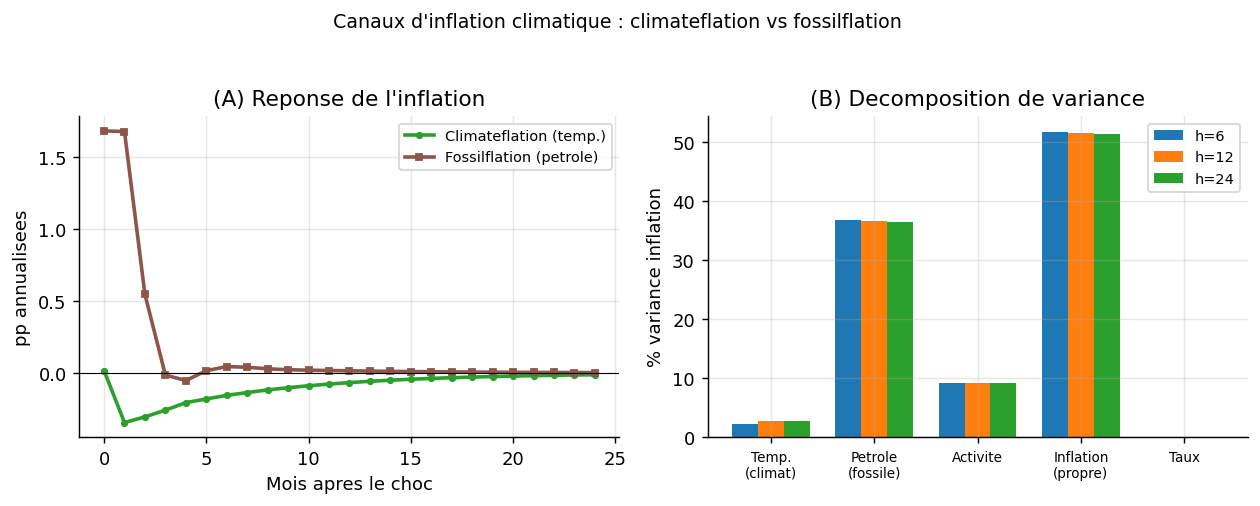
\includegraphics[width=\textwidth]{fig_channels.png}
\caption{Climateflation (choc de température) et fossilflation (choc de pétrole) dans le même
SVAR. À gauche, la réponse de l'inflation ; à droite, la part de variance expliquée. Le canal fossile
domine très largement.}
\label{fig:channels}
\end{figure}

\subsection{Une transmission qui s'intensifie}
\label{sec:res-lp}
L'effet moyen masque toutefois une dynamique temporelle déterminante.
La Figure~\ref{fig:lp} (à droite) montre que la réponse de l'inflation au choc climatique est
systématiquement plus élevée dans l'ère récente (à partir de 2007) que dans l'ère
ancienne. Le coefficient d'interaction $\gamma_h$ est positif, croissant, et
\textbf{significatif aux horizons de 14 à 18 mois} ($t$ de $2{,}1$ à $2{,}5$) : l'ère récente
ajoute de $+1{,}0$ à $+1{,}4$ pp à la réponse à moyen terme. Ce qui était neutre, voire
désinflationniste hier, devient inflationniste aujourd'hui (H3 se trouve ainsi confirmée),
une signature empirique de la \emph{climateflation} émergente, conforme aux projections de
\citet{kotz2024}.

\begin{figure}[H]
\centering
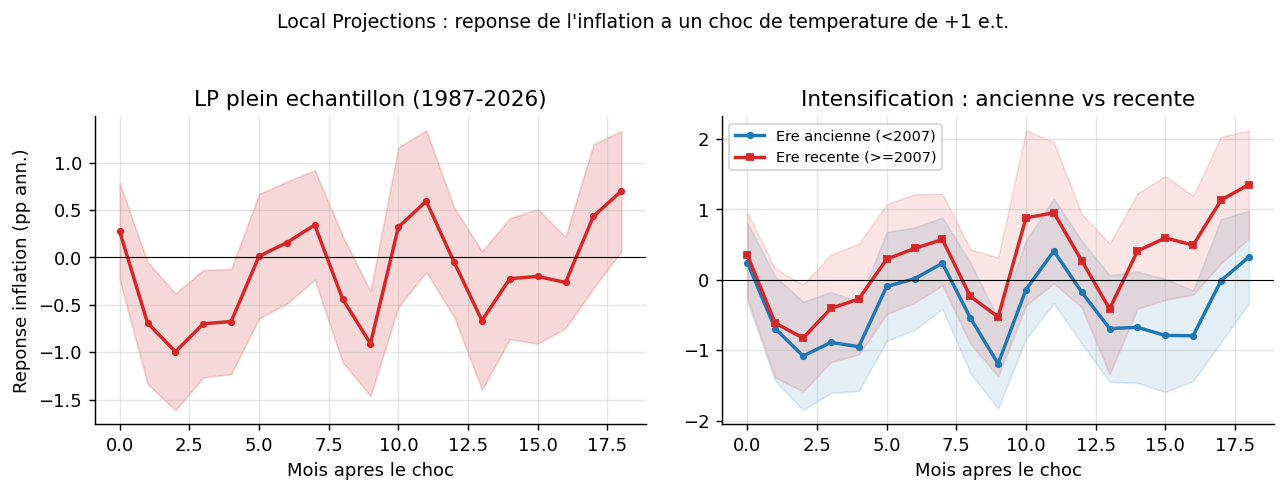
\includegraphics[width=\textwidth]{fig_lp.png}
\caption{Local Projections de l'inflation (réponse à $+1$ écart-type, HAC). À gauche, le plein
échantillon de 1987 à 2026 ; à droite, la réponse de l'ère récente (en rouge) domine nettement celle
de l'ère ancienne (en bleu).}
\label{fig:lp}
\end{figure}

\subsection{Une réponse fortement asymétrique}
\label{sec:res-nl}
La LP dépendante de l'état (Figure~\ref{fig:nl}) révèle une asymétrie marquée, conforme à H4. Les chocs
chauds (les mois plus chauds que la normale, en rouge) produisent une réponse qui devient
positive à moyen terme (de $+0{,}5$ à $+1{,}0$ pp aux horizons de 14 à 18 mois), et leur effet
cumulé sur le niveau des prix est positif ($+2{,}2$ pp à 18 mois). À l'inverse, les
chocs froids (en bleu) restent nettement désinflationnistes (avec un effet cumulé de
$-12{,}7$ pp). Cette asymétrie est cruciale pour la politique monétaire : puisque le
réchauffement multiplie les chocs chauds et raréfie les chocs froids, l'effet net du
changement climatique sur l'inflation est orienté à la hausse, même si l'effet
symétrique moyen (\S\ref{sec:res-svar}) paraît faible. Le résultat agrégé modeste et
le risque climatique réel ne sont donc pas contradictoires : ils décrivent deux moments
différents de la même distribution.

\begin{figure}[H]
\centering

\includegraphics[width=\textwidth]{fig_nonlinear.png}
\caption{Réponse asymétrique de l'inflation (LP dépendantes de l'état, 1987 à 2026). À gauche,
la réponse par horizon ; à droite, la réponse cumulée. Les chocs chauds sont inflationnistes à moyen terme,
les chocs froids désinflationnistes.}
\label{fig:nl}
\end{figure}

\subsection{Conséquences pour l'allocation d'actifs}
\label{sec:res-alloc}
La Figure~\ref{fig:assets} (à gauche) montre que les \textbf{obligations} à 10 ans sont l'actif
le plus exposé négativement au choc climatique ($\beta=-0{,}26$ pp/mois) : un choc qui tend à
être inflationniste érode mécaniquement les obligations nominales. L'\textbf{or} affiche un
bêta positif ($+0{,}26$) et joue donc un rôle de couverture, tandis que les \textbf{actions} sont
quasi neutres. Le Tableau~\ref{tab:port} en tire les conséquences : le portefeuille tangent,
lourd en obligations ($46{,}6\,\%$), porte une exposition climatique négative. Le
portefeuille \emph{climat-neutre} l'annule en délaissant les obligations
(qui passent à $36{,}3\,\%$) au profit de l'or (qui monte à $38{,}5\,\%$), au prix d'une baisse
du Sharpe de $0{,}76$ à $0{,}65$ (soit $-13{,}6\,\%$). La couverture du risque climatique a donc
un coût mesurable mais modéré.

\begin{figure}[H]
\centering
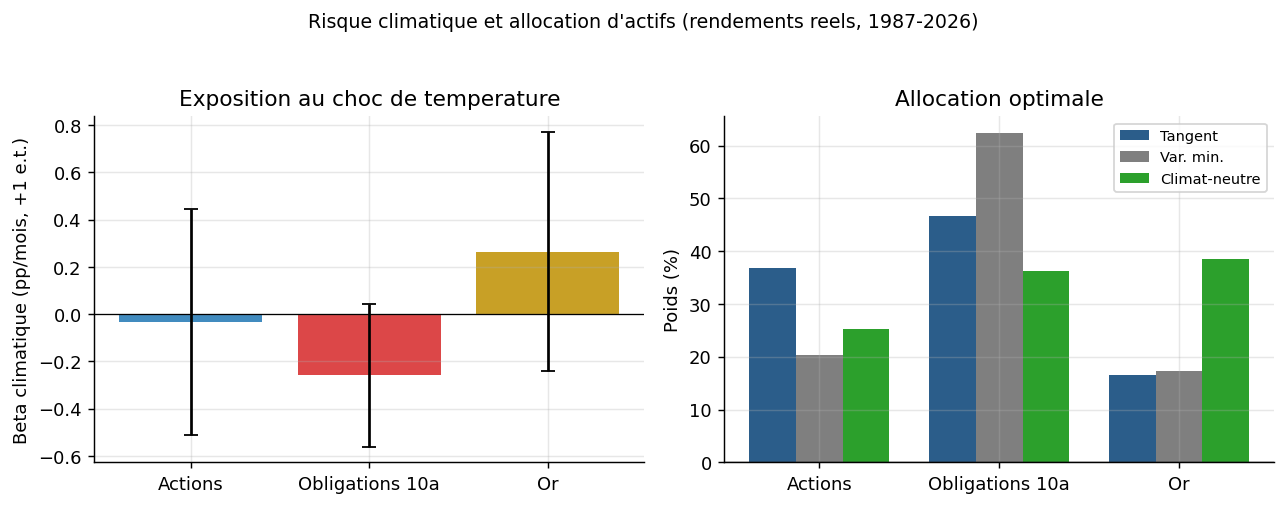
\includegraphics[width=\textwidth]{fig_assets.png}
\caption{Risque climatique et allocation (rendements réels, 1987 à 2026). À gauche, les bêtas
climatiques (barres d'erreur à 90\,\%) ; à droite, les poids des trois portefeuilles.}
\label{fig:assets}
\end{figure}

\begin{table}[H]
\centering\small
\caption{Portefeuilles optimaux et exposition climatique (rendements réels annualisés).}
\label{tab:port}
\begin{tabular}{lcccccc}
\toprule
Portefeuille & Actions & Oblig. 10a & Or & Rdt (\%) & Sharpe & $\beta$ climat \\
\midrule
Tangent (max Sharpe) & 36{,}9 & 46{,}6 & 16{,}5 & 4{,}42 & 0{,}756 & $-0{,}088$ \\
Variance minimale    & 20{,}3 & 62{,}4 & 17{,}3 & 3{,}67 & 0{,}689 & $-0{,}122$ \\
\textbf{Climat-neutre} & 25{,}2 & 36{,}3 & 38{,}5 & 3{,}97 & 0{,}654 & $\phantom{-}0{,}000$ \\
\bottomrule
\end{tabular}
\end{table}

\subsection{Robustesse}
\label{sec:robust}
Le Tableau~\ref{tab:robust} confirme que notre résultat central, à savoir un effet faible et plutôt
désinflationniste, est stable : la part de variance reste inférieure à environ $4\,\%$ et la
réponse cumulée à 12 mois demeure négative, quel que soit le nombre de retards (2, 3 ou 4),
l'ordre de Cholesky (température en premier ou en dernier) et la méthode de
détrendage. Avec un détrendage quadratique ou par filtre HP, l'effet est même plus
faible encore : ces filtres absorbent davantage de variation de basse fréquence, laissent
un choc plus net et confirment que l'effet agrégé de court terme est ténu.

\begin{table}[H]
\centering\small
\caption{Robustesse de l'effet du choc climatique sur l'inflation. FEVD(24) : part (\%) de la
variance d'inflation due au choc à 24 mois ; cum12 : réponse cumulée à 12 mois (pp).}
\label{tab:robust}
\begin{tabular}{lcc}
\toprule
Variante & FEVD(24) (\%) & cum12 (pp) \\
\midrule
Retards $p=2$ (référence) & 2{,}77 & $-2{,}02$ \\
Retards $p=3$ & 3{,}19 & $-2{,}05$ \\
Retards $p=4$ & 3{,}24 & $-2{,}11$ \\
Température ordonnée en dernier & 2{,}15 & $-1{,}84$ \\
Détrendage quadratique & 0{,}87 & $-0{,}88$ \\
Détrendage Hodrick et Prescott & 0{,}47 & $-0{,}47$ \\
\bottomrule
\end{tabular}
\end{table}

%================ 6. CONCLUSION ================
\section{Conclusion : la Banque Centrale a-t-elle un rôle à jouer ?}
Sur données américaines 1987--2026, nos six exercices économétriques dessinent une réponse
\emph{nuancée mais précise}. Le choc climatique a un effet agrégé historiquement faible sur
l'inflation ($<3\,\%$ de sa variance) et nul sur l'activité, et pèse bien moins que la
fossilflation ; mais cette transmission \emph{s'intensifie} depuis 2007, est
\emph{asymétrique} (les chocs chauds deviennent inflationnistes à moyen terme), et
\emph{reprice les actifs} en pénalisant les obligations.

\textbf{Pas (encore) une cible d'inflation directe.} L'effet agrégé symétrique étant faible
et l'activité peu affectée, une réaction mécanique du taux directeur à chaque aléa
climatique serait injustifiée : la doctrine du \emph{looking through} reste pertinente pour
les chocs ponctuels, d'autant qu'un resserrement face à un choc d'offre amplifierait la
perte d'activité. Mais l'intensification et l'asymétrie de la transmission exigent que la
banque centrale \emph{intègre le climat dans ses modèles et sa fonction de réaction},
distingue composantes transitoires et persistantes, et communique sur ces risques --- la
voie suivie par la BCE (revue stratégique, verdissement des achats d'actifs et du cadre de
garanties).

\textbf{Une contrainte institutionnelle de premier ordre.} Avant d'aller plus loin, il
convient d'être précis sur ce qu'autorise le mandat actuel. L'article~127 TFUE confie à la
BCE un objectif \emph{primaire} de stabilité des prix et un objectif \emph{secondaire} de
soutien aux politiques générales de l'Union --- parmi lesquelles la transition verte. Mais
son instrument opérationnel demeure le taux directeur, et utiliser celui-ci pour répondre à
un choc d'offre climatique est précisément le cas canonique où le \emph{looking through}
est le mieux justifié : resserrer amplifierait la perte d'activité sans éteindre la source
du choc. \emph{Dans le cadre institutionnel actuel}, la BCE ne dispose donc pas de l'outil
adapté pour cibler directement la climateflation.

\textbf{La Commission européenne comme premier acteur.} Les instruments les plus efficaces
pour internaliser le coût climatique dans les prix sont du ressort de la politique
réglementaire --- donc de la Commission et des États membres. Le Système d'Échange de
Quotas d'Émissions (SEQE/ETS), en renchérissant le carbone, agit directement sur la
\emph{fossilflation} que notre décomposition identifie comme canal dominant
($\approx 36\,\%$ de la variance d'inflation, contre $\approx 2{,}7\,\%$ pour le choc
climatique pur). La taxe carbone aux frontières (CBAM, 2023--2026) prolonge cette logique.
Ces mesures ont un effet inflationniste de court terme --- la contribution du SEQE à
l'inflation énergétique européenne est estimée à $0{,}5$--$1{,}0$ pp lors des pics de
2021--2022 --- mais elles réduisent structurellement la dépendance fossile qui, selon nos
résultats, est le principal vecteur du risque climatique sur les prix. La BCE est ici
\emph{preneur de prix} face à ces politiques : elle doit les intégrer dans ses prévisions,
non les neutraliser par le taux. Par ailleurs, le canal d'allocation (\S\ref{sec:res-alloc})
est le plus direct dès aujourd'hui : les obligations --- cœur de la transmission monétaire
et des bilans bancaires --- sont l'actif le plus vulnérable, ce qui justifie les tests de
résistance climatiques et la prise en compte du risque dans la politique de garanties.

\textbf{Vers un IPC augmenté comme condition d'un mandat élargi.} Notre analyse suggère une
piste institutionnelle de plus long terme. L'IPC mesuré aujourd'hui est un indice de prix
\emph{courants} : il ne capture pas l'inflation \emph{implicite} que le réchauffement
accumulé inscrira dans les prix futurs --- via la destruction de capital productif, la
migration des risques d'assurance vers les ménages, ou la raréfaction de ressources. Si
l'on construisait un IPC \og augmenté \fg{} intégrant une composante de coût climatique
prospectif --- prix des permis carbone, primes d'assurance ajustées au risque physique,
estimation des dommages futurs actualisés --- alors le mandat de stabilité des prix
\emph{engloberait de facto une dimension climatique}. Dans ce cadre élargi, la fonction de
réaction optimale devrait explicitement pondérer les risques de dérive inflationniste à
long terme, légitimant une réponse préventive bien au-delà du seul \emph{looking through}.

En somme, \emph{avec le mandat et les instruments actuels}, la BCE a un rôle limité mais
réel : prudentiel et de gestion des risques systémiques sur les bilans. \emph{Avec un mandat
redéfini autour d'une mesure d'inflation enrichie}, ce rôle deviendrait central. C'est moins
une question économétrique qu'un choix de gouvernance --- mais nos résultats sur
l'intensification et l'asymétrie de la transmission plaident pour que ce débat soit posé
sans attendre.

\textbf{Limites.} (i)~La variable d'activité s'arrête en 2015, ce qui borne le SVAR (le volet
LP corrige partiellement en couvrant 2026). (ii)~L'anomalie de température \emph{globale} est
un proxy : des mesures d'extrêmes \emph{locaux} (vagues de chaleur, sécheresses) seraient
plus fines. (iii)~Notre IPC est \emph{agrégé}, alors que la littérature situe l'effet sur
l'alimentation et l'énergie --- ce qui dilue probablement notre signal. (iv)~Nous ne modélisons
pas l'effet en retour des politiques climatiques (SEQE, CBAM) sur la fonction de réaction
monétaire --- ce bouclage constitue une extension naturelle.

\textbf{Extensions (par ordre de priorité).}
\begin{enumerate}[leftmargin=1.5em,itemsep=1pt,topsep=2pt]
\item \emph{Désagréger l'IPC} (alimentation/énergie via FRED ; code fourni dans
      \texttt{code/optional\_fred\_cpi.py}) : test direct du mécanisme.
\item \emph{Panel international} (économies chaudes vs tempérées) pour exploiter
      l'hétérogénéité géographique soulignée par \citet{kotz2024}.
\item \emph{Identification alternative} : restrictions de signe ou identification par
      hétéroscédasticité, pour relâcher la récursivité.
\item \emph{IPC augmenté} : construire un indice intégrant prix carbone (ETS) et primes
      d'assurance ajustées au risque physique, et ré-estimer le SVAR sur cette cible
      élargie.
\item \emph{Bouclage macro} : endogénéiser une fonction de réaction monétaire \og verte \fg{}
      dans un modèle néo-keynésien, en interaction avec un instrument de tarification du
      carbone.
\end{enumerate}

%================ BIBLIO ================
\small
\begin{thebibliography}{9}
\bibitem[Batten et al.(2020)]{batten2020} Batten, S., Sowerbutts, R., Tanaka, M. (2020).
\emph{Climate change: macroeconomic impact and implications for monetary policy.} In
\textit{Ecological, Societal, and Technological Risks and the Financial Sector}, Bank of England.
\bibitem[Faccia et al.(2021)]{faccia2021} Faccia, D., Parker, M., Stracca, L. (2021).
\emph{Feeling the heat: extreme temperatures and price stability.} ECB Working Paper No.~2626.
\bibitem[Jordà(2005)]{jorda2005} Jordà, Ò. (2005). \emph{Estimation and Inference of Impulse
Responses by Local Projections.} \textit{American Economic Review}, 95(1), 161 à 182.
\bibitem[Kotz et al.(2024)]{kotz2024} Kotz, M., Kuik, F., Lis, E., Nickel, C. (2024).
\emph{The impact of global warming on inflation: averages, seasonality and extremes.}
\textit{European Economic Review} / ECB Working Paper No.~2821.
\bibitem[Schnabel(2022)]{schnabel2022} Schnabel, I. (2022). \emph{A new age of energy
inflation: climateflation, fossilflation and greenflation.} Discours, The ECB and its
Watchers XXII Conference, Francfort, 17 mars.
\end{thebibliography}
\normalsize

\appendix
\section{Annexe : tests de stationnarité et sélection des retards}
\label{ann:adf}
\small
Tests ADF (avec sélection automatique des retards par AIC) sur l'échantillon du SVAR
(1987 à 2015). $H_0$ : présence d'une racine unitaire.
\begin{table}[H]
\centering\small
\begin{tabular}{lccc}
\toprule
Variable & Statistique ADF & $p$-value & Conclusion \\
\midrule
Choc de température & $-3{,}55$ & $0{,}007$ & stationnaire \\
$\Delta\ln$ Brent & $-5{,}87$ & $0{,}000$ & stationnaire \\
Croissance réelle & $-3{,}30$ & $0{,}015$ & stationnaire \\
Inflation & $-3{,}75$ & $0{,}003$ & stationnaire \\
$\Delta$ taux 10 ans & $-9{,}42$ & $0{,}000$ & stationnaire \\
\midrule
Taux 10 ans (niveau) & $-1{,}11$ & $0{,}711$ & non stationnaire, d'où la différenciation \\
\bottomrule
\end{tabular}
\end{table}
Pour la sélection des retards du VAR, l'AIC et le FPE retiennent $p=2$, tandis que le BIC et le HQIC, plus
parcimonieux, retiennent $p=1$. Nous retenons $p=2$ (AIC) et vérifions en
\S\ref{sec:robust} que les résultats restent stables pour $p \in \{2,3,4\}$. Le système estimé
est stable (le module minimal des racines vaut $1{,}15$, supérieur à 1).

\textbf{Reproductibilité.} L'ensemble des résultats, figures et tableaux est reproductible
via \texttt{python run\_all.py} (voir \texttt{README.md}). Chaque script, numéroté de
\texttt{01} à \texttt{07}, correspond à une étape de notre démarche.
\normalsize

\end{document}